\documentclass{llncs}
\usepackage[ngerman]{babel}
\usepackage{float}
\usepackage{graphicx}

\begin{document}

\title{Starjumper}
\author{Robert Strobl, Johannes Albrecht, Tim Berning, Stefan H\"artel}
\institute{Hasso-Plattner-Institut, Prof.-Dr.-Helmert-Str. 2-3, 14482 Potsdam}

\maketitle

\section{Einleitung}

\subsection{Spielprinzip}
Starjumper ist ein Renn- und Geschicklichkeitsspiel, bei dem der Spieler mit einem
Raumschiff \"uber eine hindernisreiche Strecke mit diversen Abgr\"unden fahren und
schlussendlich sicher ins Ziel gelangen muss.\\
Dabei besitzen die Fl\"achen der Streckenabschnitte unterschiedliche Eigenschaften,
die sich auf das Fahrverhalten des Raumschiffs auswirken k\"onnen, z.B. Abbremsen
des Spielers.\\
Die Steuerung umfasst Beschleunigen, Bremsen, Lenken nach links oder rechts und
Springen.

\subsection{Spielidee}
Vorlage f\"ur unser Spiel war der Spieleklassiker Skyroads aus dem Jahr 1993, welches
von Bluemoon entwickelt wurde und wiederum selbst eine Neuauflage des Spiels Kosmonaut
aus dem eigenen Hause darstellte.\\
Das Spielprinzip wurde f\"ur Starjumper gr\"o\ss tenteils \"ubernommen.


\section{Steuerung}
Die Steuerung des Raumschiffs erfolgt sehr intuitiv, der Spieler kann beschleunigen,
bremsen, lenken und springen. Die folgende Tabelle zeigt die in-game Tastaturbelegung:

\begin{table}[H]
	\begin{center}
		\begin{tabular}{|c|c|}
			\hline
			Beschleunigen & Pfeiltaste oben \\
			\hline
			Bremsen & Pfeiltaste unten \\
			\hline
			Links & Pfeiltaste links \\
			\hline
			Rechts & Pfeiltaste rechts \\
			\hline
			Springen & Leertaste \\
			\hline
		\end{tabular}
	\end{center}
	\caption{Tastaturbelegung}
\end{table}
\noindent Dar\"uber hinaus kann per \texttt{Escape} jederzeit aus dem Spiel in das Levelauswahlmen\"u
gewechselt werden. Im Hauptmen\"u beendet ein Druck auf \texttt{Escape} das Programm.\\
Die Navigation im Men\"u erfolgt \"uber die Pfeiltasten, die ausgew\"ahlte Strecke wird mit \texttt{Enter} gestartet.


\section{Architektur}

\textit{Die Beschreibung der Architektur erfolgt in kleineren logischen Einheiten, eine Gesamt\"ubersicht
aller verwendeten Klassen und ihrer Verbindungen untereinander findet sich am Ende des Dokuements.}\\
Im Folgenden sollen nun die wichtigsten architektonischen Bestandteile von Starjumper
erl\"autert werden.

\subsection{LevelMenu}
Das \texttt{LevelMenu} bildet den Einstiegspunkt des Spiels. Es bietet eine \"Ubersicht der verf\"ugbaren
Levels, die selektiert und gestartet werden k\"onnen. Bei Instanziierung parst das \texttt{LevelMenu} die
XML-Dateien, in denen die Levels des Spiels definiert wurden, und bereitet sie f\"ur die weitere Verarbeitung auf.\\
Selektiert der Benutzer ein Level, alloziiert \texttt{LevelMenu} eine Instanz der Klasse \texttt{Level} und
\"ubergibt die aufbereiteten Inhalte des entsprechenden Levelfiles. Anschlie\ss end ersetzt \texttt{Level}
das \texttt{LevelMenu} als zu rendernden Szenengraphen.\\
Hier wird au\ss erdem der Keyboardhandler definiert, der die Logik der Escape-Taste umsetzt (Programm beenden
bzw. aus dem laufenden Spiel zur Level\"ubersicht zur\"uckkehren), und in den \texttt{Viewer} eingeh\"angt.\\

\begin{figure}[H]
	\centering
	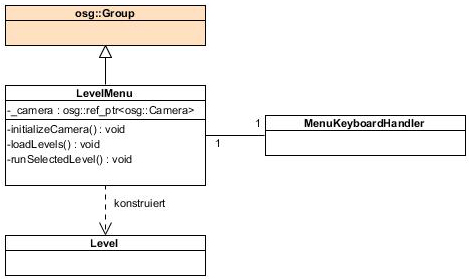
\includegraphics[width=1\textwidth]{LevelMenu.jpg}
	\caption{Klassendiagramm LevelMenu}
\end{figure}

\subsection{Level}
Die von \texttt{osg::Group} erbende Klasse \texttt{Level} stellt in sich den zu einem Spiel geh\"orenden Szenengraphen
dar und verbindet alle Teile der Spiellogik. \texttt{Level} erstellt aus den \"ubergebenen Leveldaten eine Reihe
von Levelelementen (Kuboiden, Tunnel, ...), den \texttt{Player} (dies gilt nur f\"ur die erste Levelinstanz aufgrund der Singleton Eigenschaft, siehe Abschnitt zum Player),
das \texttt{HeadUpDisplay}, den Kameramanipulator und k\"ummert sich um die Beleuchtung.\\
Neben den OpenSceneGraph-Komponenten erstellt und verwaltet \texttt{Level} zudem die Bullet Physics World, innerhalb
derer physikalische Simulationen parallel zu OSG ablaufen.\\

\begin{figure}[H]
	\centering
	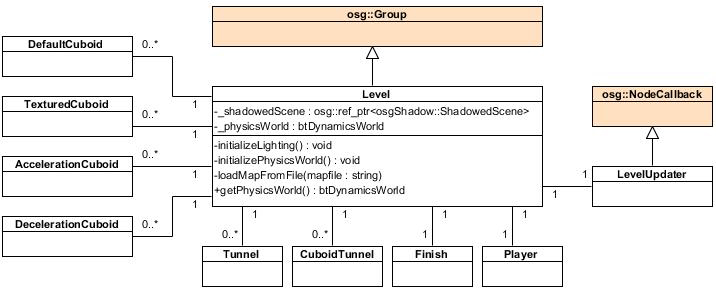
\includegraphics[width=1\textwidth]{Level.jpg}
	\caption{Klassendiagramm Level}
\end{figure}

\subsection{Player}
\texttt{Player} stellt die vom Benutzer steuerbare Entit\"at dar in Form eines Raumschiffs, das fix aus einer Datei
geladen wird. Zwecks Positionierbarkeit wird das Model in einer PositionAttitudeTransform gekapselt.
Neben dem Laden dieser Modeldatei werden in \texttt{Player} die Physikkomponenten f\"ur den Spieler generiert.
Die Interaktion des Benutzers mit dem Spiel erfolgt \"uber die Komponenten \texttt{PlayerState} und \texttt{PlayerUpdater},
die im n\"achsten Abschnitt n\"aher erl\"autert werden.\\
\textit{Details zu \texttt{KinematicCharacterController} und \texttt{btGhostObject} in Kombination finden sich im Abschnitt "Designentscheidungen".}

\begin{figure}[H]
	\centering
	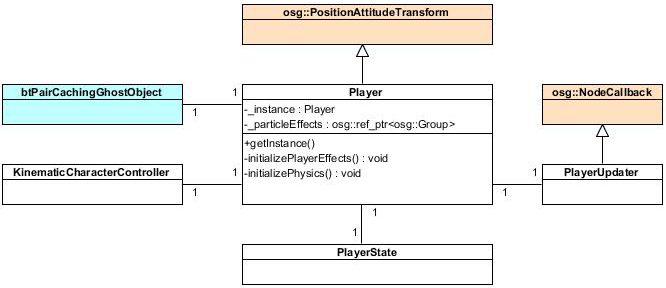
\includegraphics[width=1\textwidth]{Player.jpg}
	\caption{Klassendiagramm Player}
\end{figure}

\section{Designentscheidungen und Design Patterns}
Dieser Abschnitt besch\"aftigt sich mit einigen Besonderheiten der Starjumper Implementierung und erl\"autert deren
Beweggr\"unde und Vorteile gegen\"uber alternativer Implementierungsstrategien.

\subsection{Physik}
Da sich die physikalischen Effekte, die sich in Starjumper wiederfinden (sollten), auf korrekte Auswirkung der Schwerkraft
beim Sprung oder dem Verlassen einer Plattform, sowie der Erkennung von Kollisionen mit Umgebungsobjekten beschr\"anken,
stand zu Beginn die \"Uberlegung im Raum, diese von Hand zu implementieren. Schnell wurde jedoch klar, dass trotz des
an sich geringen Umfangs der Anforderungen an die Physik eine manuelle Implementierung viel Zeit kosten w\"urde, und so fiel
die Entscheidung zugunsten der Verwendung der Physikbibliothek Bullet.\\
Die von Bullet zur Verf\"ugung gestellten Klassen \texttt{btKinematicCharacterController} und \texttt{btGhostObject} boten
laut Interface genau die gew\"unschten Funktionen: Das Ghost Object agiert als Rigid Body in der Physikwelt und kennt
zu jedem Zeitpunkt alle eventuell vorhandenen Kollisionspartner, der \texttt{btKinematicCharacterController} stellt ein
Steuerungsinterface f\"ur das GhostObject zur Verf\"ugung. Aufgrund einiger weniger Unzul\"anglichkeiten musste allerdings
der Controller angepasst werden, sodass statt dem \texttt{btKinematicCharacterController} eine modifizierte Version
namens \texttt{KinematicCharacterController} Verwendung findet.\\
Das Rendering durch OpenSceneGraph und die Physik laufen parallel. So ist zu erkl\"aren, dass beispielsweise f\"ur
Streckenelemente wie \texttt{Cuboid} jeweils eine Repr\"asentation f\"ur den Szenengraphen und ein \texttt{btRigidBody}
f\"ur die Physics World existiert. Die Kommunikation zwischen diesen beiden Entit\"aten findet im \texttt{PlayerUpdater}
statt. Korrekt parametrisiert (Bewegungsrichtung, Fallgeschwindigkeit, Gravitation) berechnet der Controller bei jedem
Stepping der Physics World die neue Position des Spielers, welche anschlie\ss end durch den \texttt{PlayerUpdater}
abgefragt und auf die \texttt{PositionAttitudeTransform} des Spielermodells \"ubertragen wird. Im Gegenzug werden
durch den Benutzer per Tastendruck im \texttt{PlayerState} gesetzte Requests - wie der Wunsch nach links zu steuern -
ausgewertet und dienen als Basis f\"ur die Aktualisierung der Parameter des Controllers.

\subsection{Player}
Der \texttt{Player} bzw. sein Modell wird in jeder Levelinstanz ben\"otigt. Die im Verlauf des Spiels vorgenommenen \"Anderungen
am \texttt{Player} beschr\"anken sich jedoch auf Transformationen der umgebenden \texttt{PositionAttitudeTransform} und sind leicht reversibel,
wie am Beispiel des Reset erkennbar ist. In einer fr\"uheren Version wurde f\"ur jedes Level eine neue Instanz der Klasse
erzeugt, die logischerweise das Laden des Modells beinhaltet, was zu erheblicher Verz\"ogerung des Spielstarts f\"uhrte.\\
Auf Basis dieser Erkenntnisse wurde ein Refactoring vorgenommen und der \texttt{Player} zu einem Singleton erweitert. Das hei\ss t,
dass das Spielermodell nur noch ein einziges Mal beim Starten des Programms geladen werden muss und als global verf\"ugbare
Ressource gehandhabt wird, ein Aufruf der statischen Methode \texttt{Player::getInstance()} liefert auf Wunsch die Player-Instanz.
Die initiale Erzeugung des \texttt{Player} Objekts erfolgt beim ersten Aufruf dieser Funktion.\\
Neben dem Wegfall der Ladezeiten erm\"oglicht dies dar\"uber hinaus den globalen Zugriff auf den Zustand des Spielers,
der z.B. die an verschiedenen Stellen des Spiels ben\"otigten Eigenschaften Geschwindigkeit und Neigungswinkel enth\"alt.

\subsection{ParticleEffectFactory}
Die Erstellung von Partikeleffekten erfordert diverse Komponenten und deren Konfiguration. So ist neben einem \texttt{ParticleSystem}, das
die einzelnen Partikel \"uber die Dauer ihres Bestehens einschlie\ss lich ihrer L\"oschung verwaltet, ein entsprechender
\texttt{ParticleSystemUpdater} n\"otig - ein Callback, der das kontinuierliche Stepping des Partikelsystems \"ubernimmt. Weitere Komponenten
sind ein \texttt{Emitter}, der - bestehend aus einem \texttt{Shooter} und einem \texttt{Placer} - f\"ur die initiale Platzierung der Partikel verantwortlich
ist, und ein sogenanntes \texttt{Program}, das sich beliebig konfigurieren l\"asst und das Verhalten der Partikel steuert.\\
All diese Komponenten gilt es f\"ur jeden Partikeleffekt zu erstellen, woraus sich in h\"ochstem Ma\ss e redundanter Code erg\"abe
Um diesem entgegenzuwirken, existiert in Starjumper eine Klasse \texttt{ParticleEffectFactory}. Dem Factory Pattern folgend stellt sie Methoden
bereit, die einen durch die Klasse \texttt{ParticleEffect} gekapselten Partikeleffekt erzeugen und je nach Situation konfigurieren.\\
\texttt{ParticleEffect} implementiert eine Art "Standard"-Partikeleffekt, dessen einzelne Komponenten und weitere Einstellungen sich
durch im Konstruktor \"ubergebene Objekte \"uberschreiben lassen. Durch diese Aufteilung wird duplizierter Code vermieden und
gleichzeitig die Verantwortung f\"ur das Erstellen von Partikeleffekten an einem Ort konzentriert.


\section{Diskussion und Ausblick}
Die relativ simpel gehaltene Klassenhierarchie und minimale Bindung zwischen den Komponenten hat sich w\"ahrend der Entwicklung als
vorteilhaft erwiesen. Der Einflussbereich einer Klasse beschr\"ankt sich in der Regel auf sie selbst, sowie die von ihr erstellen
Kindknoten des Szenengraphen. So k\"onnen \"Anderungen an Klassen vorgenommen werden, (fast) ohne die \"ubrige existierende Funktionalit\"at
zu beeinflussen. Auch das Ausnutzen der von OpenSceneGraph bereitgestellten M\"oglichkeiten wie Update Callbacks oder Event Handler, die
bei der Traversierung des Szenengraphen nacheinander aufgerufen werden, spart an einigen Stellen Code.\\
Ein zweifelhaftes Implementierungsdetail ist die Verwendung des Viewers als globale Variable. Auf den Viewer wird an diversen Stellen
zugegriffen, sodass dessen Verf\"ugbarkeit nicht optional war. Genauso wenig optimal war jedoch der Ansatz, eine Referenz auf den
Viewer durch alle Ebenen durchzureichen, sodass schlussendlich die Entscheidung auf die Variante der globalen Variable fiel.

\newpage

\appendix

\section{Komplettes Klassendiagramm}

\begin{figure}[ht]
	\centering
	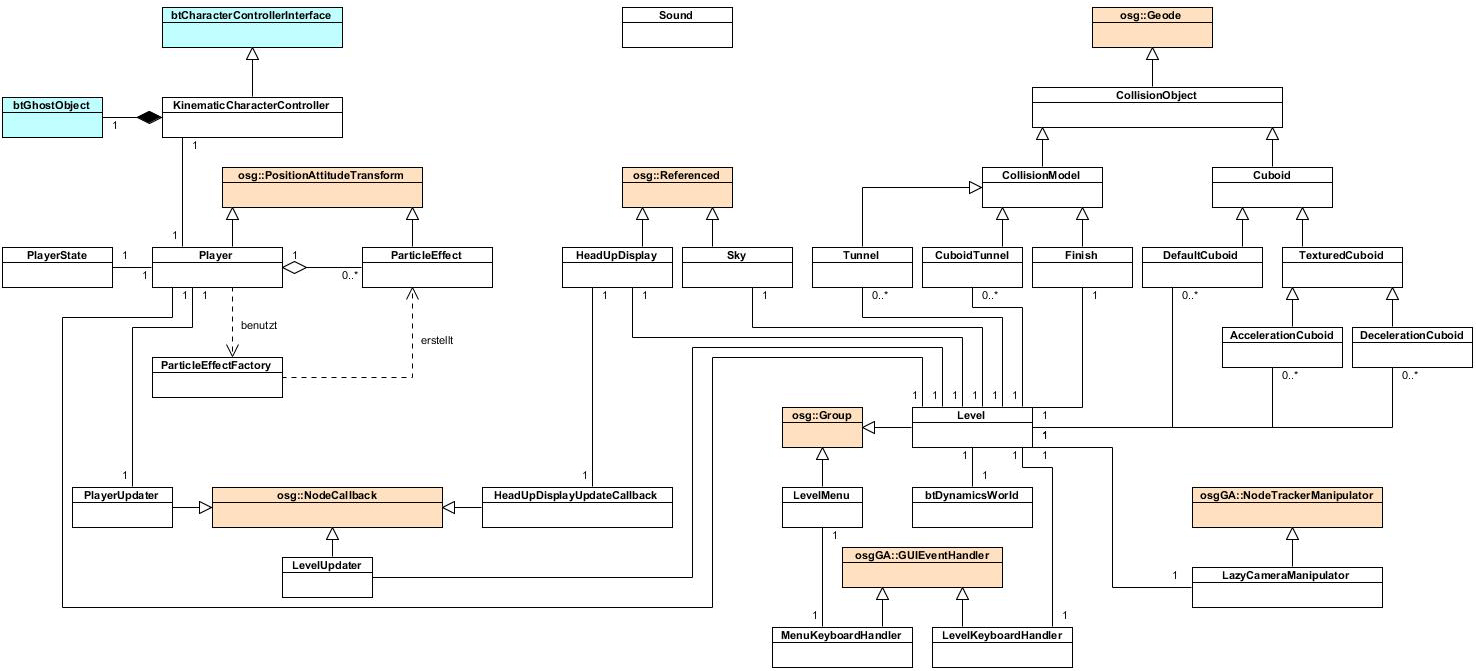
\includegraphics[width=1.6\textwidth, angle=-90]{All.jpg}
	\caption{Klassendiagramm komplett}
\end{figure}


\end{document}